%! Author = jannikeschler
%! Date = 18/09/2022

\documentclass[reprint,english,notitlepage]{revtex4-2}
\usepackage{amsmath}
\usepackage[mathletters]{ucs}
\usepackage[utf8x]{inputenc}
\usepackage[english]{babel}
\usepackage{esint}
\usepackage{physics,amssymb}
\usepackage{graphicx}
\usepackage{xcolor}
\usepackage{hyperref}
\usepackage{listings}
\usepackage{subfigure}
\hypersetup{
    colorlinks,
    linkcolor={red!50!black},
    citecolor={blue!50!black},
    urlcolor={blue!80!black}}

\lstset{inputpath=,
	backgroundcolor=\color{white!88!black},
	basicstyle={\ttfamily\scriptsize},
	commentstyle=\color{magenta},
	language=Python,
	morekeywords={True,False},
	tabsize=4,
	stringstyle=\color{green!55!black},
	frame=single,
	keywordstyle=\color{blue},
	showstringspaces=false,
	columns=fullflexible,
	keepspaces=true}

\begin{document}
\title{Simulating Planetary orbits of a solar system}
\author{Jannik Eschler \& Oskar Idland}
\date{\today}
\affiliation{Institute of Theoretical Astrophysics, University of Oslo}

\begin{abstract}
This is an abstract \colorbox{red}{Complete this summary at the end of the paper}
\end{abstract}
\maketitle

\section{Introduction}
When making our way out of the earth's atmosphere, we will have to know where our destination will be after the launch.
To be able to reach our destination we therefore have to get known in our solar system and explore and simulate the different planets in the system.
After finding out the orbits of the planets, it will be much easier to coordinate our launch to our target to minimize the time and effort required to find the destination.
Using this, we will also be able to give estimates about the possibility of extraterrestrial life discovering our solar system.

\section{Method}
The calculation of the planetary orbits in our solar system can either be done numerically or analytically.
Both methods have their advantages and disadvantages compared to the other.
To be able to find the analytical orbit of a planet, we will first have to find an analytical expression for the orbit of a planet.
As planetary orbits usually are ellipses with the star positioned in one of the two foci of the ellipse, we will be able to derive a formula for the position of the planet based on the formula for and ellipse.
An ellipse is defined as "A closed plane curve generated by a point moving in such a way that the sums of its distances from two fixed points is a constant." \colorbox{red}{Merriam Webster}
The analytical expression for an ellipse in cartesian coordinates with the origin in the middle is given by
\begin{align}
    \frac{x^2}{a^2} + \frac{y^2}{b^2} = 1 \label{ellipse_analytic_cart}
\end{align}
For the calculations in this report, it is however advantageous to be able to use this expression in polar coordinates.
When switching to polar coordinates, we will be using the distance $r = |\textbf{r}|$ from the star in one focus point to the point on the ellipse and the angle $f$ at the star from the semi-major axis to the vector $\textbf{r}$ as seen in figure \ref{fig:Ellipse_fig}.
In orbital mechanics, the angle $f$ is also often called the true anomaly.
\begin{figure}[h]
	%% h(here), t(top of page), b(bottom of page)
	\centering
	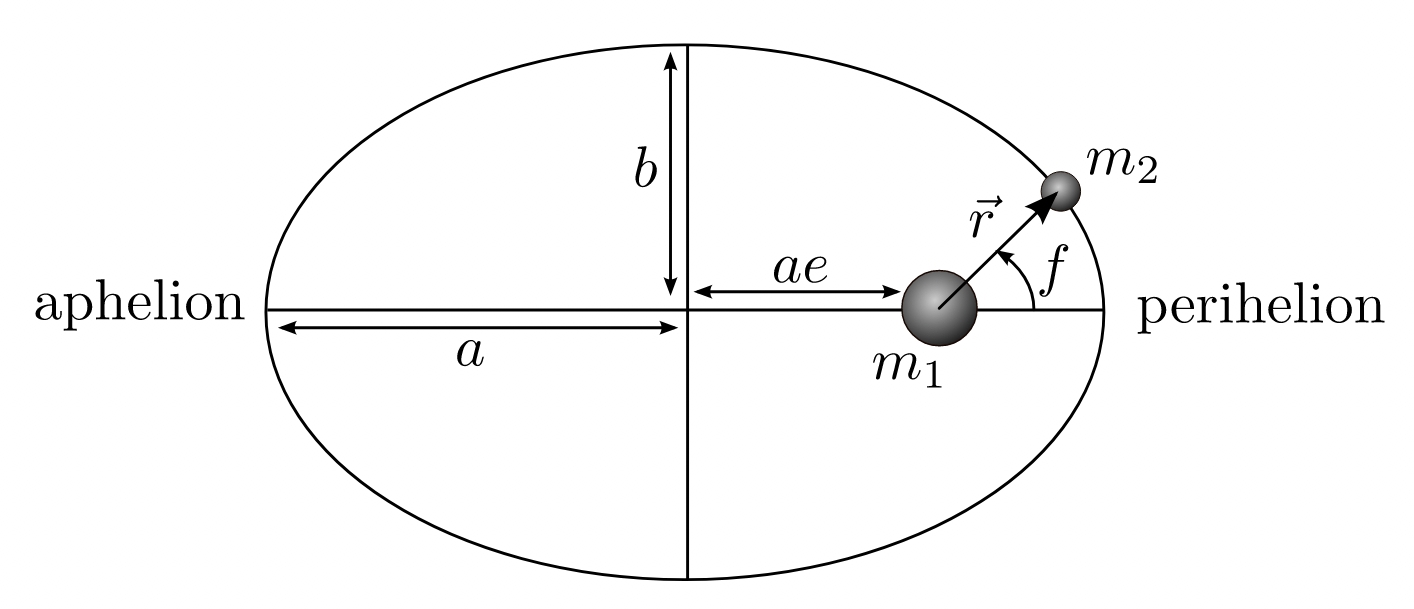
\includegraphics[scale=0.3]{Figures/Ellipse}
	\caption{Figure of an ellipse with all major components}\label{fig:Ellipse_fig}
\end{figure}
Based on figure~\ref{fig:Ellipse_fig} we are now able to see that
\begin{align}
    &x = ae + r\,cos(f) \label{x_ellipse}\\
	&y = r\,sin(f) \label{y_ellipse}
\end{align}
Using equations~\ref{x_ellipse} and~\ref{y_ellipse} we wre now able to find an equation for the distance $r$
\begin{align*}
    r = \frac{a(1-e^2)}{1 + e\,cos(f)}
\end{align*}
with e being the eccentricity of the ellipse given by
\begin{align*}
    e = \sqrt{1-\frac{b^2}{a^2}}
\end{align*}
Here, a is the semi-major axis and b is the semi-minor axis of the ellipse.
Now, $r$ can be used to convert the coordinates back to cartesian coordinates using equations~\ref{x_ellipse} and~\ref{y_ellipse}.
By iterating over a collection of equally spaced values between $0$ and $2\pi$, we will find collection of points on the elliptical orbit of the planets, which can then be plotted.
When repeating this for each planet using the given constants for each planet, we will be able to simulate the orbits or all planets.\\\\
The analytical expression, can be used to find the orbit of a given planet, but not the velocity or the position of the planet on the orbit the planet at a given time.
To find the position of the planet in the orbit as a function of time, we will first need to simulate the orbit numerically.
The general idea of the simulation is to use newtons second law $\sum\textbf{F} = m\textbf{a}$ to calculate the acceleration of the planet at a certain position.
In this simulation, all forces except gravitational forces from the star will be neglected.
Therefore the total force exerted on the planet can be calculated using Newtons law of universal gravitation.
\begin{align*}
    &\sum\textbf{F} = G\,\frac{m_1 m_2}{r^2} \label{Newton_Grav_law}\\
	&\sum\textbf{F} = m_1 \textbf{a}\\
	&\bold{a} = G\,\frac{m_1}{r^2}
\end{align*}
With $G$ being the gravitational constant, $m_1$ being the mass of the star, $m_2$ being the mass of the planet, and $r$ being the distance between the star and the planet.\\\\
Using the initial velocity of the object at the position we are calculating the acceleration for, as well as the acceleration, we can find the velocity after a small time interval $\Delta t$.
Correspondingly, using the initial position and velocity, the position after the time step $\Delta t$ can be calculated.
The process is then repeated using the new position and velocity to calculate the acceleration in the point and velocity and position after another time interval $\Delta t$.
There are different variations of this process, with different advantages and disadvantages.\\
In this simulation the Leapfrog method will be used.
This method calculates the acceleration in a point and uses it to find the velocity $\textbf{v}_h$ after $ \frac{dt}{2}$.
Velocity $\textbf{v}_h$ and the initial position of the planet will then be used to calculate the new position after a time interval $\Delta t$.\\
\begin{figure}[h]
	%% h(here), t(top of page), b(bottom of page)
	\centering
	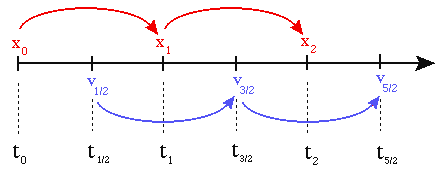
\includegraphics[scale=0.4]{Figures/leapfrog1}
	\caption{\colorbox{red}{Visualisation of the Leapfrog integration algorithm}}\label{fig:Leapfrog_vis}
\end{figure}\\
As $\textbf{v}_h$ is somewhere between the velocity of the object in the initial position and the position after a time interval $\Delta t$, the calculation of the new position will be more exact.
The process can be described using three equations:
\begin{align*}
    \textbf{a}_i &= A(\textbf{x}_i)\\
	\textbf{v}_{i+1/2} &= \textbf{v}_{i-1/2} + \textbf{a}_i\,\Delta t\\
	\textbf{x}_{i} &= \textbf{x}_i + \textbf{v}_{i+1/2}\,\Delta t
\end{align*}
After simulating the orbits of the planets, the results can be used to find a function of time approximating the orbit of each planet.
This will be done by interpolating the results into a function.\\\\

To examine and test the orbits for inaccuracies, we can make use of Johannes Kepler's laws of planetary motion.
The three laws state:
\begin{enumerate}
    \item The orbit of a planet is an ellipse with the
		Sun in one of the foci.
	\item A line connecting the Sun and the planet
		sweeps out equal areas in equal time intervals.
	\item The orbital period around the Sun and the
		semimajor axis of the ellipse are related through:
		\begin{align*}
		    P^2 = a^3
		\end{align*}
		\colorbox{red}{where P is the period in years and a is the
		semimajor axis in Astronomic Units}
\end{enumerate}

First, we will check whether our results agree with Kepler's second law.
To do this, two areas on different sides of the orbit of our home planet,which have been swept out in the same time interval will be compared.\\
To calculate the areas, each area will be divided into smaller areas $dA$, which can be determined by using formula~\eqref{Kepler_dArea}.
\begin{align}
    dA = \frac{1}{2}r^2 d\theta \label{Kepler_dArea}
\end{align}
\colorbox{red}{The derivation of this formula can be found in the Appendix}
When running the simulation, a small area $dA$ which is equal to the area swept out by the position vector $\textbf{r}$ during the time interval $\Delta t$, will be calculated using formula~\eqref{Kepler_dArea}.
To find the total area swept out during a time interval $[a, b]$, all smaller areas $dA$ in the interval $[a, b]$ need to be added together.
This will give an approximation of the total swept out area.
The simulation will calculate the area at two different places in the orbit.
One around the point where the planet is closest to the start, called perihelion, and one around the point the furthest away from the star, called aphelion.\\
The areas should look different, as the planet will have the highest angular velocity at the perihelion and lowest angular velocity at the perihelion.
This is due to the spin of the planet around the star being conserved.
The covered distance and mean velocity of the planet during the interval $[a, b]$, are therefore also interesting measurements, which will be calculated in the simulation.
To do this, the small distances $\Delta \textbf{r}$ which are covered by the planet in the small time intervals $\Delta t$ in the interval $[a, b]$ will therefore be added together.
This will yield in the total distance traveled by the planet in the time interval $[a, b]$.
The mean velocity is found by dividing the total distance by the time $t = b-a$.\\

Furthermore we will check if the orbits are consistent with Kepler's third law~\eqref{Kepler3} as well as Newtons revised version of Kepler's third law~\eqref{KeplerNewton3}.
Since we have found the rotational period of each planet around the sun using the simulation, we will only have to calculate the rotational period of each planet using Kepler's third law and Newtons revised version and compare them to find out how well they agree.
\begin{align}
    P^2 &= a^3 \label{Kepler3}\\
	P^2 &= \frac{4 \pi^2}{G \left( m_1 + m_2 \right)} a^3 \label{KeplerNewton3}
\end{align}



\section{Results}
\subsection{Planetary Orbits}
    The simulation of the orbits yielded in both numeric and analytic orbits for all planets.
	For both the analytic and the numeric orbits, arrays containing the velocity and position of each planet at \colorbox{red}{N} equally spaced positions along the orbit are returned.
	The simulation then created figure~\ref{fig:Orbit_Plot} from these arrays.
\begin{figure}[h]
	%% h(here), t(top of page), b(bottom of page)
	\centering
	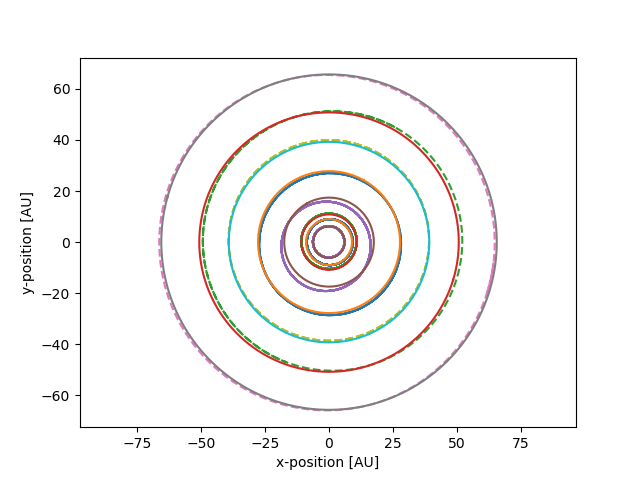
\includegraphics[scale=0.4]{Figures/Orbit_plots}
	\caption{Plot of the simulated orbits of our solar system}\label{fig:Orbit_Plot}
\end{figure}\\
	The star is denoted by the black dot in the middle of the solar system.
	Around the star, there are 8 sets of orbits, one set for each planet.
	The numeric orbit for each planet is represented by a dashed line, whereas the analytic orbis is represented by a solid line.\\
	The numeric and analytic orbits are slightly elliptic, and line up quite well for all planets, with only some deviance.
	As seen in Figure~\ref{fig:Orbit_Plot}, they have the same shapes, but appear not to be entirely concentric.

\subsection{Comparison to Kepler's Laws}
	To compare the orbit of our home planet to Kepler's second law, two different areas $A$ swept out by the position vector $ \textbf{r}$ during the same time interval have been calculated.
	Furthermore, the covered distance and mean velocity during each time interval have been calculated and are shown in table~\ref{tab:Kepler2_table1}.
	The differences between the values of each area are presented in table~\ref{tab:Kepler2_table2}. Areas are given in AU$^2$, Distances in AU and Velocities in AU/Yr.
\begin{table}[h]
	%% l (Left aligned), c (Centered), r (Right aligned)
    \begin{tabular}{ |c|c|c| }
		\hline
        Planet 0 & Aphelion & Perihelion\\
        \hline
        Area & 0.00000307 & 0.00000307\\
        \hline
		Distance & 6.823815E-07 & 6.823823E-07\\
		\hline
		Velocity & 0.20996355 & 0.20996378\\
		\hline
    \end{tabular}
	\caption{Area, Distance and Velocity results for calculated areas at Aphelion and Perihelion}
	\label{tab:Kepler2_table1}
\end{table}

\begin{table}[h]
    \begin{tabular}{ |c|c| }
		\hline
		 & Difference\\
		\hline
		Area & 3.181500E-12 AU^2\\
		\hline
		Distance & 7.306208E-13 AU\\
		\hline
		Velocity & 0.00000022 AU/Yr\\
		\hline
	\end{tabular}
    \caption{Differences between results of the two areas}
    \label{tab:Kepler2_table2}
\end{table}\\

	To check whether the calculated orbits agree with Kepler's third law and Newton's revised version of Kepler's third law, the orbital period has been calculated analytically and using each of the two laws~\eqref{Kepler3} and~\eqref{KeplerNewton3} for each planet.
	This yields in the following results.\\

        \hline
		Planet 0 \tab\tab\tab\tab hello\\
        Analytic	12.81499 Yrs\\
		Kepler		27.00534 Yrs\\
		Newton		12.81498 Yrs\\
		Difference	14.19036 Yrs\\
        \hline

		Planet 1\\
        Analytic	16.93432 Yrs\\
		Kepler		35.68609 Yrs\\
		Newton		16.93431 Yrs\\
		Difference	18.75177 Yrs\\
        \hline

		Planet 2\\
        Analytic	34.83863 Yrs\\
		Kepler		73.41629 Yrs\\
		Newton		34.83862 Yrs\\
		Difference	38.57766 Yrs\\
        \hline

		Planet 3\\
        Analytic	252.32753 Yrs\\
		Kepler		531.73585 Yrs\\
		Newton		252.32499 Yrs\\
		Difference	279.41086 Yrs\\
        \hline

		Planet 4\\
        Analytic	116.61089 Yrs\\
		Kepler		245.73693 Yrs\\
		Newton		116.61089 Yrs\\
		Difference 	129.12603 Yrs\\
        \hline

		Planet 5\\
        Analytic	69.47113 Yrs\\
		Kepler		146.39819 Yrs\\
		Newton		69.47113 Yrs\\
		Difference 	76.92706 Yrs\\
        \hline

		Planet 6\\
        Analytic	171.66819 Yrs\\
		Kepler		361.76050 Yrs\\
		Newton		171.66798 Yrs\\
		Difference	190.09252 Yrs\\
        \hline

		Planet 7\\
        Analytic	7.25601 Yrs\\
		Kepler		15.29077 Yrs\\
		Newton		7.25601 Yrs\\
		Difference	8.03475 Yrs\\
        \hline

\\It can be seen that the orbits are not entirely consistent with Kepler's third law.
The relative difference is approximately $110.733 \pm 0.001\%$ for all planets.
They are however very consistent with Newton's revised version of Kepler's third law as they deviate less than $0.0015\%$ from each other.
The relative difference here is approximately $0.0005 \pm 0.001\%$ for all planets, which is very accurate.
\section{Discussion}
To get an accurate simulation, the time interval dt needs to be sufficiently small.
An adequate number is approximately 10'000 steps per year of simulation, which corresponds to a time interval of $\Delta t = 52$ min $33.6$ sec.
Using smaller time intervals will result in a more precise simulation, but will increase computing time.
	\subsection{Subsection}

\section{Conclusion}
And the conclusion


\section{References}
References are important!\\
1:\:https://www.merriam-webster.com/dictionary/ellipse\\
2:\:https://cvarin.github.io/CSci-Survival-Guide/leapfrog.html\\
3:\:https://www.uio.no/studier/emner/matnat/astro/AST2000/h22/undervisningsmateriell/lecture_notes/part1b.pdf

\section{Appendix: Mathematical Derivations}
	\subsection{Section 1}
	\begin{align*}

	\end{align*}

\end{document}